\chapter{A Didática do Abstrato}


Thomás de Aquino, em sua obra \emph{De veritate}, argumenta que o conhecimento humano começa com a percepção sensorial do mundo concreto, mas alcança sua plenitude ao transcender o particular e abraçar o universal através da abstração. Esse processo de abstração é fundamental para a matemática e a ciência da computação, onde conceitos complexos são frequentemente representados por meio de símbolos e estruturas que vão além da experiência direta.


Grafos e digrafos são simultaneamente concretos (nós e arestas) e abstratos (propriedades globais como cortes, conectividade, laminaridade). A multiplicidade de noções (caminhos, ciclos, cortes, componentes, condensação) \cite{bondy2008graph,diestel2017graph,west2001introduction}. Essas noções exigem transitar entre níveis de representação (intuitivo, visual, simbólico, formal) \cite{tall1991advanced}, o que pode ser desafiador. A abstração é poderosa, mas também pode ser uma barreira: conceitos como “corte ativo” ou “complementaridade primal–dual” são difíceis de visualizar e internalizar sem apoio didático adequado.


Então, como ensinar e aprender conceitos abstratos de forma eficaz? O ensino de matemática no ensino superior, especialmente em áreas como teoria dos grafos parecem sofrer com dificuldades específicas. A seguir, discutimos essas dificuldades e como o uso de ferramentas visuais e interativas pode ajudar a superá-las.

\section{Fundamentos cognitivos e didáticos}

O ensino de matemática no ensino superior exige transitar entre registros de representação (intuitivo, visual, simbólico, formal) com intencionalidade didática \cite{tall1991advanced}. À luz da teoria da carga cognitiva, é útil distinguir: (i) a \emph{carga intrínseca}, determinada pela complexidade dos esquemas a construir e pelos pré-requisitos ativados; (ii) a \emph{carga extrínseca}, criada pela forma de apresentação; e (iii) a \emph{carga pertinente} (\emph{germane}), isto é, o esforço dedicado à organização e automatização de esquemas \cite{sweller1988cognitive}. Em cursos avançados, a extrínseca cresce quando definições, símbolos e figuras não são co-referenciados no tempo e no espaço, dificultando a coordenação entre o que se lê, o que se vê e o que se infere.

\subsection{Desafios centrais}
Aprender conteúdos de alta abstração envolve lidar com sobrecarga cognitiva intrínseca e extrínseca \cite{sweller1988cognitive}. Diretrizes de aprendizagem multimídia indicam que combinar representações verbais e visuais pode reduzir carga desnecessária e favorecer integração semântica \cite{mayer2009multimedia,paivio1990}. Em matemática avançada, a transição entre níveis de representação (intuitivo, formal, simbólico) exige mediação cuidadosa \cite{tall1991advanced} e atenção a como exemplos, contraexemplos e invariantes são apresentados.


No caso específico de algoritmos com provas baseadas em complementaridade primal--dual, é frequente que estudantes compreendam os passos operacionais sem internalizar a estrutura teórica que garante correção e otimalidade.

\subsection{Lidando com grafos e digrafos}
Na prática, o que mais dificulta o ensino de digrafos não é definir vértices e arcos, mas articular o que fazemos localmente com as estruturas globais que sustentam as provas de correção e de otimalidade em arborescências de custo mínimo — em particular, nos métodos de Chu–Liu/Edmonds e de Frank —: cortes ativos, componentes fortemente conexas (SCCs) e famílias laminares de conjuntos \cite{bondy2008graph,diestel2017graph,west2001introduction}. Quando essa articulação não aparece, cresce a \emph{carga intrínseca} (múltiplas dependências simultâneas) e também a \emph{carga extrínseca} (o esforço de alinhar texto, fórmulas e figuras). Nesse contexto específico destacamos três desafios didáticos:
\begin{itemize}\setlength{\itemsep}{2pt}
    \item \textbf{Articular o local com o global:} escolher a melhor aresta de entrada para cada vértice não garante coerência global; isso pode criar ciclos. Ver o grafo \emph{condensado} em SCCs (cada ciclo vira um ``bloco'') torna esse efeito visível e manipulável (Fig.~\ref{fig:didatica-condensado}). \emph{Dificuldade típica:} estudantes tendem a projetar a heurística local para o todo e se surpreendem com ciclos “inesperados” — uma fonte comum de sobrecarga por conflito entre intuições locais e restrições globais.
    \item \textbf{Acompanhar efeitos de contração/expansão:} contrair um ciclo (substituí\-lo por um supervértice) e depois reexpandir impacta os custos reduzidos \(c'\) e os cortes que ficam ``ativos''. A laminaridade — cortes aninhados, sem interseções conflitantes — fornece uma geometria simples para seguir essas mudanças (Fig.~\ref{fig:didatica-laminar}). \emph{Dificuldade típica:} perder o fio entre representações (grafo original, condensado, reexpansão) aumenta a carga extrínseca; sinalizar o que mudou em cada etapa reduz esse atrito.
    \item \textbf{Mapear o ``fazer do algoritmo'' para a linguagem primal–dual:} ações como elevar potenciais, escolher entradas e contrair ciclos correspondem a garantias teóricas. Em particular, \emph{apertude} (custo reduzido zero) e \emph{complementaridade} (exatamente uma aresta entra em cada conjunto ativo) certificam a otimalidade. Relacionar essas ideias às métricas que coletamos (tempos, número de contrações, pico de memória) ajuda a ligar prática e teoria, via custos reduzidos e reexpansão (Figs.~\ref{fig:didatica-reduced-cost} e \ref{fig:didatica-reexpansion}). \emph{Dificuldade típica:} executar os passos sem ver como eles tornam certas restrições “justas” dificulta a internalização do porquê; explicitar os vínculos entre ação e certificação reduz a distância entre o operacional e o conceitual.
\end{itemize}


No exemplo da figura abaixo, a condensação do digrafo \(D\) em \(D_0\) torna visível a relação entre escolhas locais (entradas por vértice) e estrutura global (ciclos, cortes). Cada SCC (bloco) pode ser tratado como uma unidade, facilitando a compreensão de como ciclos surgem e são resolvidos. Apesar de não ser suficiente para ilustrar situações mais complexas, essa visualização ajuda criar intuição sobre a atualização de custos reduzidos e a dinâmica de contração/expansão.

\begin{figure}[H]
    \centering
    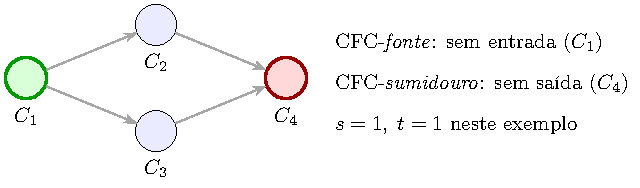
\includegraphics[width=.72\linewidth]{figures/fig_condensado_st.pdf}
    \caption{Condensação de $D_0$ e fontes do DAG: ver o grafo “como” blocos (SCCs) ajuda a articular o local (entradas por vértice) com o global (cortes e contrações).}
    \label{fig:didatica-condensado}
\end{figure}

\section{Visualização e interação: princípios em uso}
Há evidências de que diagramas e animações, quando bem projetados, podem acelerar a compreensão de relações topológicas e causais \cite{larkin1987diagram,ware2012information}.


A teoria da carga cognitiva sugere que combinar representações verbais e visuais pode reduzir carga extrínseca e favorecer integração semântica \cite{mayer2009multimedia,paivio1990}. Diretrizes de aprendizagem multimídia recomendam evitar excesso de elementos visuais que não contribuam para o entendimento (reduzindo carga extrínseca) e alinhar texto e imagens no tempo e no espaço (reduzindo esforço de coordenação) \cite{mayer2009multimedia}.


No campo específico de matemática avançada, Tall enfatiza a coordenação entre registros — intuitivo, visual, simbólico e formal — como motor da passagem do pensamento predominantemente procedimental para o conceitual \cite{tall1991advanced}. Diagramas não são meros adornos: estruturam inferências espaciais e relacionais de modo mais eficiente que sentenças lineares \cite{larkin1987diagram}.



Na educação em ciência da computação, visualizações de algoritmos têm efeito positivo sobretudo quando promovem \emph{engajamento ativo} (prever, manipular, explicar) e não apenas consumo passivo \cite{hundhausen2002meta,naps2003engagement}.

\section{Disseminação de conteúdos avançados: o ecossistema de ferramentas}


Materiais que conectam teoria, evidências empíricas e interatividade têm maior potencial de transferência e retenção.


Tendo em vista esses fundamentos, ferramentas digitais podem ajudar a reduzir carga extrínseca e a integrar registros (visual, simbólico, formal) quando a interação é desenhada para promover \emph{engajamento ativo} \cite{mayer2009multimedia,sweller1988cognitive,hundhausen2002meta,naps2003engagement}. A seguir, apresentamos categorias de ferramentas úteis no ensino de grafos, indicando finalidades, forças e limitações, e posicionamos a nossa aplicação nesse ecossistema.

\subsection{Ferramentas didáticas no ensino de teoria dos grafos}

Várias ferramentas digitais podem apoiar o ensino de grafos e digrafos, cada uma com forças e limitações específicas. A seguir, discutimos quatro categorias principais: (i) diagramas programáveis e tipografia matemática, (ii) exploração e edição de grafos, (iii) visualização de algoritmos, e (iv) ambientes programáveis e reprodutibilidade.

\subsubsection{Diagramas e matemática}

Algumas ferramentas permitem criar diagramas de grafos com semântica visual consistente, integrando-os a textos matemáticos. Essas ferramentas são úteis para ilustrar conceitos, definições e provas em materiais didáticos.


Ambientes como Graphviz/dot e TikZ/PGF permitem especificar grafos declarativamente e gerar figuras reprodutíveis com layouts consistentes \cite{graphviz,tantau2015tikz}. Benefícios didáticos: (i) semântica visual estável (mesmo conceito, mesma forma), (ii) autoria próxima ao símbolo e ao texto (co-referência), (iii) manutenção e versionamento fáceis. Limitações: a interação costuma ser offline (figuras estáticas) e a curva de aprendizado de sintaxe pode ser um obstáculo inicial. Em contextos de prova e definição, esses recursos ancoram a narrativa formal com diagramas que obedecem às diretrizes de \cite{larkin1987diagram,ware2012information}.


Contudo, diagramas estáticos não capturam a dinâmica de algoritmos que envolvem mudanças estruturais (elevação de potenciais, contração/expansão, seleção de arestas). Para isso, são necessárias ferramentas interativas que permitam explorar essas transformações em tempo real.

\subsubsection{Exploração e edição de grafos}

Ferramentas de exploração e edição de grafos permitem que os usuários interajam com representações gráficas de dados, facilitando a manipulação e a análise de estruturas complexas. Essas ferramentas são essenciais para atividades que exigem uma compreensão profunda das relações entre os elementos de um grafo.



Dentre elas destacam-se Gephi, yEd e Cytoscape, que oferecem layouts automáticos, filtros e medidas de rede \cite{bastian2009gephi,yed,shannon2003cytoscape}. São adequadas para: (i) reconhecer padrões estruturais (componentes, comunidades), (ii) discutir implicações de layouts para percepção de estruturas, (iii) atividades de descoberta assistida (``\textit{overview} \textrightarrow{} \textit{filter} \textrightarrow{} \textit{details}'') \cite{shneiderman1996eyes}. Limitações: (i) foco em análise exploratória de dados, não em algoritmos específicos; (ii) carga extrínseca ao alternar entre interface gráfica e conceitos teóricos; (iii) falta de controle fino sobre estados intermediários de algoritmos.

\subsubsection{Visualização de algoritmos}

Existem diversas ferramentas dedicadas à visualização de algoritmos, que ilustram passo a passo como um algoritmo opera sobre uma estrutura de dados.


Repositórios e portais como VisuAlgo e iniciativas similares apresentam animações de algoritmos clássicos com controle do ritmo e de estados \cite{visualgo,hundhausen2002meta,naps2003engagement}. Evidências sugerem ganhos quando o estudante prevê, manipula e explica o que vê, ao invés de consumir animações passivamente. Pontos de atenção: (i) alinhar a animação às noções teóricas subjacentes (invariantes, certificados), (ii) explicitar mapeamentos entre ``o que acontece'' e ``o que se garante'' (p.ex., custo reduzido zero \(c'=0\), complementaridade), (iii) evitar excesso de elementos visuais que aumentem carga extrínseca \cite{mayer2009multimedia}.

\subsubsection{Ambientes programáveis e reprodutibilidade}

Ferramentas como Jupyter Notebooks e bibliotecas como NetworkX permitem combinar código, texto e visualizações em um único documento interativo \cite{kluyver2016jupyter,hagberg2008networkx}. Essas ferramentas são valiosas para criar exemplos reprodutíveis e explorar algoritmos de forma prática.


Contudo, requerem familiaridade com programação e podem introduzir carga extrínseca se o foco se desviar para detalhes de implementação. A curadoria do conteúdo é essencial para manter o foco didático e evitar dispersão.


Tendo em vista essas categorias, desenvolvemos uma aplicação \textit{web} interativa que combina elementos de visualização de algoritmos e ambientes programáveis, com foco específico nos algoritmos de arborescência de custo mínimo. A seguir, apresentamos princípios envolvendo a teoria de interação humano-computador que orientaram o desenho da ferramenta, e em seguida descrevemos a aplicação com seus respectivos detalhes de implementação e como ela se posiciona nesse ecossistema.

